\subsection{Greedy Best-First Search}
\noindent Greedy Best-First Search (GBFS) is an informed search algorithm that selects the next node based on a heuristic function. Unlike A*, it considers only the estimated cost to the goal and ignores the cost incurred so far. This makes it faster but less optimal, as it can get trapped in local optima. GBFS is often used when a fast, approximate solution is needed rather than the absolute shortest path.

\begin{figure}[H]
	\centering
	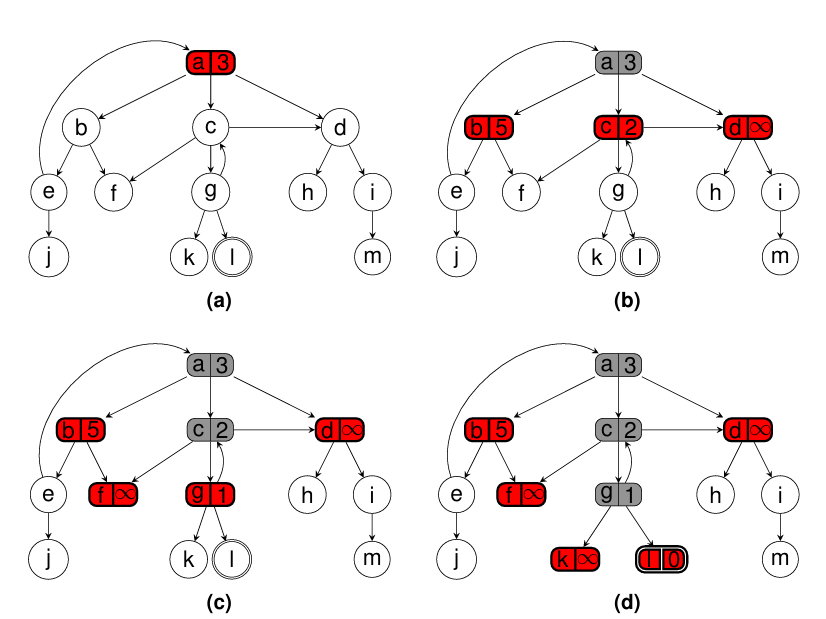
\includegraphics[width=0.8\textwidth]{./imgs/gbfs.png}
	\caption{Greedy Best-First Search}
	\label{fig:GBFS}
\end{figure}

\subsubsection{Pseudocode}
\begin{algorithm}[H]
	\caption{Greedy Best-First Search (\textit{start, goal, heuristic})}
	\label{alg:gbfs}
	\begin{algorithmic}[1]
		\State priority queue \(\gets\) [(start, heuristic(start))]
		\While {priority queue is not empty}
		\State node \(\gets\) dequeue(priority queue)
		\If {node = goal}
		\State return path
		\EndIf
		\ForAll {neighbor in valid moves}
		\If {neighbor not visited}
		\State mark neighbor as visited
		\State enqueue(priority queue, (neighbor, heuristic(neighbor)))
		\EndIf
		\EndFor
		\EndWhile
		\State return failure
	\end{algorithmic}
\end{algorithm}

\subsubsection{Implementation}
\begin{itemize}
	\item \textbf{\_\_init\_\_(\ldots)}
	      Initializes the Greedy Best-First Search (GBFS) algorithm with grid dimensions, matrix representation, initial player position, stone positions, and switch positions. It also includes options for deadlock detection and heuristic optimization.

	\item \textbf{search()}
	      Implements the GBFS algorithm using a priority queue (min-heap). The function explores states by selecting the one with the lowest heuristic \( h \), without considering the cost \( g \). It expands nodes by generating successors, updating costs, and maintaining a hash table for efficient state lookup.

	\item \textbf{handle(new\_state, closed, frontier, state\_hash\_table)}
	      Manages newly generated states, checking if they should be added to the frontier or updated in the hash table based on their heuristic values.

	\item \textbf{heuristic(stones\_pos, switches\_pos)}
	      Computes the heuristic function to estimate the cost to reach the goal. It selects between the Hungarian heuristic and Manhattan heuristic based on the optimization flag.

	\item \textbf{mahattan\_heuristic(stones\_pos, switches\_pos)}
	      Calculates the heuristic using the Manhattan distance, summing up the minimum distances from each stone to a switch.

	\item \textbf{hungarian\_heuristic(stones\_pos, switches\_pos)}
	      Uses the Hungarian algorithm to optimally assign stones to switches, minimizing the total weighted Manhattan distance.

	\item \textbf{can\_go(current\_state, dir)}
	      Checks whether the player can move in a given direction from the current state without encountering obstacles.

	\item \textbf{go(current\_state, dir, heuristic)}
	      Generates a new state by moving the player in the specified direction, updating positions and recalculating heuristic values.

	\item \textbf{construct\_path(final\_state)}
	      Reconstructs the sequence of moves leading to the goal state by backtracking from the final state.

\end{itemize}

\subsubsection{Time and Space Complexity}
\textbf{Time Complexity:} \( O(b^d) \), where \( d \) is the depth of the solution. GBFS does not guarantee optimality and may explore irrelevant paths.

\textbf{Space Complexity:} \( O(b^d) \), as it stores all visited states.
